\chapter{RBFNN-based identification on an example network}
\label{NN_based_example}

\emph{In Appendix F. a numerical example of the system identification is carried out on a simple network.}

\section{The example network in EPANET}
\label{example1_EPANET}

The reason for testing the identification method on data from a simple EPANET model is that, in simulation, several different operations of the network can be studied. On a real world network, typically the operation or control cannot be taken to its extremes, as this would mean undesired service to the customers . Therefore, the network shown in \figref{fig:epanet_example1_id} has been created to mimic the behaviour of a multi-inlet, single-WT system, such that the identification method, presented in \chapref{identification_design} is being tested. 

%EPANET example network for identification
\begin{figure}[H]
\centering
%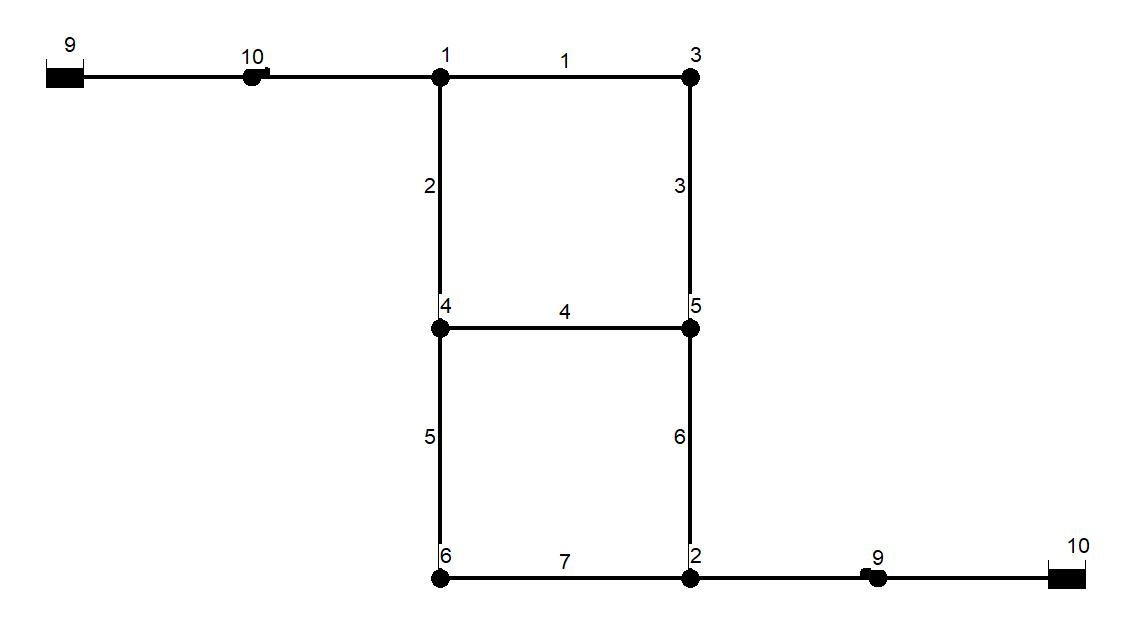
\includegraphics[width=0.6\textwidth]{report/pictures/example1_epanetmodel}
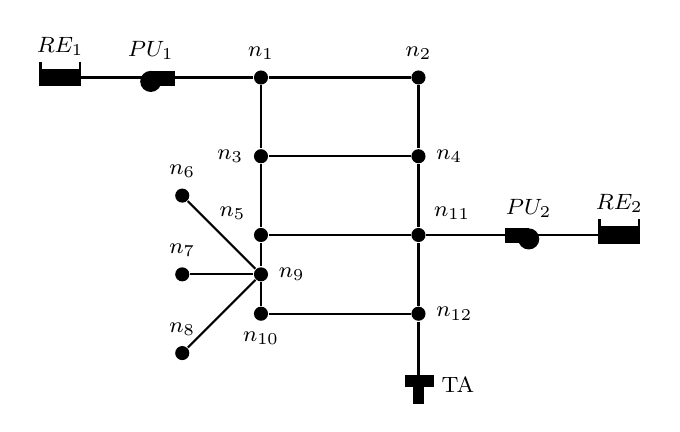
\begin{tikzpicture}[semithick,state/.style ={ draw,shape=circle,scale=0.9}]

\node[circle,fill,inner sep=1.8pt,label=above : \footnotesize$n_1$] (A) at (0,0) {};
\node[circle,fill,inner sep=1.8pt,label=above : \footnotesize$n_2$] (B) at (2,0) {};
\node[circle,fill,inner sep=1.8pt,label= left: \footnotesize$n_3$] (C) at (0,-1) {};
\node[circle,fill,inner sep=1.8pt,label= right: \footnotesize$n_4$] (D) at (2,-1) {};
\node[circle,fill,inner sep=1.8pt,label= above right: \footnotesize $n_{11}$] (E) at (2,-2) {};
\node[circle,fill,inner sep=1.8pt,label= above left: \footnotesize$n_5$] (F) at (0,-2) {};
\node[circle,fill,inner sep=1.8pt,label= below : \footnotesize$n_{10}$] (G) at (0,-3) {};
\node[circle,fill,inner sep=1.8pt,label=  right: \footnotesize$n_9$] (H) at (0,-2.5) {};
\node[circle,fill,inner sep=1.8pt,label=  right: \footnotesize$n_{12}$] (I) at (2,-3) {};
\node[circle,fill,inner sep=1.8pt,label=  above: \footnotesize$n_6$] (J) at (-1,-1.5) {};
\node[circle,fill,inner sep=1.8pt,label=  above: \footnotesize $n_7$] (M) at (-1,-2.5) {};
\node[circle,fill,inner sep=1.8pt,label=  above: \footnotesize $n_8$] (L) at (-1,-3.5) {};



\draw [thick] (A) --  (B) node[above  =0.05 cm] {\footnotesize$$};
\path (A) edge [thick]  node[left  =0.05 cm] {\footnotesize$$} (C);
\path (B) edge [thick] node[right  =0.05 cm] {\footnotesize$$} (D);
\path (C) edge [thick] node[above  =0.05 cm] {\footnotesize$$} (D);
\path (C) edge [thick] node[left  =0.05 cm] {\footnotesize$$} (F);
\path (D) edge [thick] node[right  =0.05 cm] {\footnotesize$$} (E);
\path (E) edge [thick] node[below  =0.05 cm] {\footnotesize$$} (F);
\path (F) edge [thick] node[below  =0.05 cm] {\footnotesize$$} (H);
\path (H) edge [thick] node[below  =0.05 cm] {\footnotesize$$} (G);
\path (H) edge [thick] node[below  =0.05 cm] {\footnotesize$$} (J);
\path (H) edge [thick] node[below  =0.05 cm] {\footnotesize$$} (M);
\path (H) edge [thick] node[below  =0.05 cm] {\footnotesize$$} (L);
\path (G) edge [thick] node[below  =0.05 cm] {\footnotesize$$} (I);
\path (E) edge [thick] node[below  =0.05 cm] {\footnotesize$$} (I);

%PU2
\node[circle,fill,inner sep=2.7pt,label= above : \footnotesize $ PU_2$] (I) at (3.4,-2.05) {};
\draw [thin,fill] (3.1,-1.92) rectangle (3.4,-2.1);


\begin{scope}[xscale=-1,yscale=1]
%PU1
\node[circle,fill,inner sep=2.7pt,label= above : \footnotesize $ PU_1$] (I) at (3.4-2,-2.05+2) {};
\draw [thin,fill] (3.1-2,-1.92+2) rectangle (3.4-2,-2.1+2);

\end{scope}

\draw [thick](2.1,-2) -- (3.1,-2);
\draw [thick, fill] (1.84,-3.79) rectangle (2.18,-3.92);
\draw [thick,fill] (1.95,-3.92) rectangle (2.06,-4.13);
\draw [thick](2,-3.1) -- (2,-3.8);
\node at (2.5,-3.9) {\footnotesize TA};


\draw [thick](-0.1,0) -- (-1.1,0);


\draw [thick](3.5,-2) -- (4.3,-2);
\draw [thick](-1.5,0) -- (-2.3,0);
\draw [thick](-2.3,0.2) -- (-2.3,-0.1) -- (-2.8,-0.1) -- (-2.8,0.2);
\draw [thick,fill] (-2.8,0.1) rectangle (-2.3,-0.1);
\draw [thick](4.3,-1.8) -- (4.3,-2.1) -- (4.8,-2.1) -- (4.8,-1.8);
\draw [thick,fill] (4.3,-1.9) rectangle (4.8,-2.1);
\node at (-2.55,0.4) {\footnotesize $RE_1$};
\node at (4.55,-1.6) {\footnotesize $RE_2$};
\end{tikzpicture} 
\caption{Multi-inlet, Single-WT example network.}
\label{fig:epanet_example1_id}
\end{figure}
\vspace{-3mm}

The network shown in \figref{fig:epanet_example1_id} consists of two pumping stations $PU_1$ and $PU_2$ and a Water Tank $TA$. Furthermore, reservoirs are present in the network, as in EPANET reservoirs are required for simulating pumps. These reservoirs $RE_1$ and $RE_2$ are different from WTs in the sense that they cannot be emptied in the simulation. Additionally, the physical and operational properties of the network can be found in \appref{physical_properties_example1}. 

The controls implemented on the network are based on simple time scheduling of the two pumping stations. Both pumps turn off when the pressure head in the WT is above $19.85 [m]$. $PU_2$ turns on again if the pressure head in the WT decreases to $19.55 [m]$. Furthermore, $PU_2$ turns on again only if the pressure head in node $n_1$ exceeds $43 [m]$. The initial pressure head in the WT is $19.5 [m]$.

\section{Identification and validation of the output equation}
\label{identification_and_validation_of_the_output_eq} 

The identification is carried out on the simulation data, exported from EPANET. In order to validate the identified model, scenarios with increased and decreased consumption patterns are taken intro account. It is worth noting, that the control properties of the network are kept the same, as any modification in control would mean a new operating point in the WSS. Thus, the model is tested by modifying the total demand and therefore creating different inlet pressure and flow settings for the two pumping stations. The identification is carried out on the network when the total consumption is $\sigma_1$. The validation is done when the total consumption is increased($\sigma_2$) and when decreased($\sigma_3$), respectively. Furthermore, all three consumption curves are periodic with a time period of 24 hours, however the validation has been done on a 72 hours long test data. \figref{fig:sigma123} shows the three different consumption patterns.

  %Total consumptions
 \begin{figure}[H]
 \centering
 %\hspace{0mm}
 %
\includegraphics[width=0.35\textwidth]{report/pictures/missingfigure}
 % This file was created by matlab2tikz.
%
%The latest updates can be retrieved from
%  http://www.mathworks.com/matlabcentral/fileexchange/22022-matlab2tikz-matlab2tikz
%where you can also make suggestions and rate matlab2tikz.
%
\definecolor{mycolor1}{rgb}{0.00000,0.44700,0.74100}%
\definecolor{mycolor2}{rgb}{0.85000,0.32500,0.09800}%
\definecolor{mycolor3}{rgb}{0.92900,0.69400,0.12500}%
%
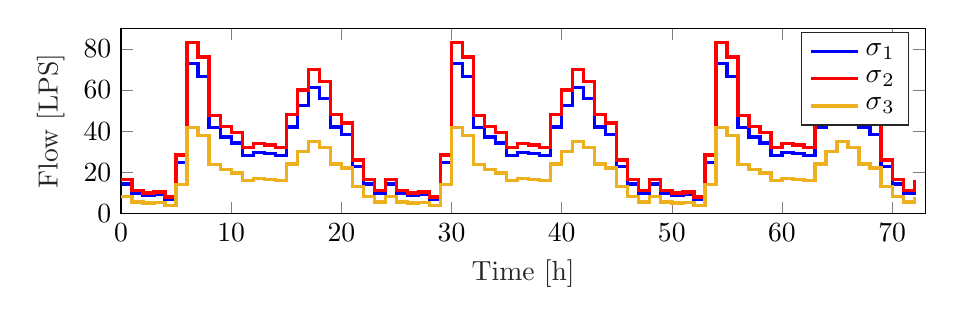
\begin{tikzpicture}

\begin{axis}[%
width=4.021in,
height=0.926in,
at={(0.758in,0.481in)},
scale only axis,
xmin=0,
xmax=73,
xlabel style={font=\color{white!15!black}},
xlabel={Time [h]},
ymin=0,
ymax=90,
ylabel style={font=\color{white!15!black}},
ylabel={Flow  [LPS]},
axis background/.style={fill=white},
legend style={legend cell align=left, align=left, draw=white!15!black}
]
\addplot[const plot, color=blue, line width=1.2pt] table[row sep=crcr] {%
0	14.35\\
1	9.8\\
2	8.75\\
3	9.1\\
4	7\\
5	24.85\\
6	72.8\\
7	66.5\\
8	41.65\\
9	37.1\\
10	34.3\\
11	28\\
12	29.75\\
13	29.05\\
14	28\\
15	42\\
16	52.5\\
17	61.25\\
18	56\\
19	42\\
20	38.5\\
21	22.75\\
22	14.35\\
23	9.8\\
24	14.35\\
25	9.8\\
26	8.75\\
27	9.1\\
28	7\\
29	24.85\\
30	72.8\\
31	66.5\\
32	41.65\\
33	37.1\\
34	34.3\\
35	28\\
36	29.75\\
37	29.05\\
38	28\\
39	42\\
40	52.5\\
41	61.25\\
42	56\\
43	42\\
44	38.5\\
45	22.75\\
46	14.35\\
47	9.8\\
48	14.35\\
49	9.8\\
50	8.75\\
51	9.1\\
52	7\\
53	24.85\\
54	72.8\\
55	66.5\\
56	41.65\\
57	37.1\\
58	34.3\\
59	28\\
60	29.75\\
61	29.05\\
62	28\\
63	42\\
64	52.5\\
65	61.25\\
66	56\\
67	42\\
68	38.5\\
69	22.75\\
70	14.35\\
71	9.8\\
72	14.35\\
};
\addlegendentry{$\sigma{}_\text{1}$}

\addplot[const plot, color=red, line width=1.2pt] table[row sep=crcr] {%
0	16.4\\
1	11.2\\
2	10\\
3	10.4\\
4	8\\
5	28.4\\
6	83.2\\
7	76\\
8	47.6\\
9	42.4\\
10	39.2\\
11	32\\
12	34\\
13	33.2\\
14	32\\
15	48\\
16	60\\
17	70\\
18	64\\
19	48\\
20	44\\
21	26\\
22	16.4\\
23	11.2\\
24	16.4\\
25	11.2\\
26	10\\
27	10.4\\
28	8\\
29	28.4\\
30	83.2\\
31	76\\
32	47.6\\
33	42.4\\
34	39.2\\
35	32\\
36	34\\
37	33.2\\
38	32\\
39	48\\
40	60\\
41	70\\
42	64\\
43	48\\
44	44\\
45	26\\
46	16.4\\
47	11.2\\
48	16.4\\
49	11.2\\
50	10\\
51	10.4\\
52	8\\
53	28.4\\
54	83.2\\
55	76\\
56	47.6\\
57	42.4\\
58	39.2\\
59	32\\
60	34\\
61	33.2\\
62	32\\
63	48\\
64	60\\
65	70\\
66	64\\
67	48\\
68	44\\
69	26\\
70	16.4\\
71	11.2\\
72	16.4\\
};
\addlegendentry{$\sigma{}_\text{2}$}

\addplot[const plot, color=mycolor3, line width=1.2pt] table[row sep=crcr] {%
0	8.2\\
1	5.6\\
2	5\\
3	5.2\\
4	4\\
5	14.2\\
6	41.6\\
7	38\\
8	23.8\\
9	21.2\\
10	19.6\\
11	16\\
12	17\\
13	16.6\\
14	16\\
15	24\\
16	30\\
17	35\\
18	32\\
19	24\\
20	22\\
21	13\\
22	8.2\\
23	5.6\\
24	8.2\\
25	5.6\\
26	5\\
27	5.2\\
28	4\\
29	14.2\\
30	41.6\\
31	38\\
32	23.8\\
33	21.2\\
34	19.6\\
35	16\\
36	17\\
37	16.6\\
38	16\\
39	24\\
40	30\\
41	35\\
42	32\\
43	24\\
44	22\\
45	13\\
46	8.2\\
47	5.6\\
48	8.2\\
49	5.6\\
50	5\\
51	5.2\\
52	4\\
53	14.2\\
54	41.6\\
55	38\\
56	23.8\\
57	21.2\\
58	19.6\\
59	16\\
60	17\\
61	16.6\\
62	16\\
63	24\\
64	30\\
65	35\\
66	32\\
67	24\\
68	22\\
69	13\\
70	8.2\\
71	5.6\\
72	8.2\\
};
\addlegendentry{$\sigma{}_\text{3}$}

\end{axis}
\end{tikzpicture}% 
 \vspace{-2.5mm}
 \caption{Consumption patterns used for identification and validation.}
 \label{fig:sigma123}
 \end{figure}

 \vspace{-3mm}

 The inlet flows of the two pumping stations $PU_1$ and $PU_2$, and the WT pressure $\hat{p}$ are shown in \figref{fig:WT_sigma1}. 

 \vspace{-3mm}

   %Inlet flow - sigma1
 \begin{figure}[H]
 \centering
 %\hspace{0mm}
 %
\includegraphics[width=0.35\textwidth]{report/pictures/missingfigure}
 % This file was created by matlab2tikz.
%
%The latest updates can be retrieved from
%  http://www.mathworks.com/matlabcentral/fileexchange/22022-matlab2tikz-matlab2tikz
%where you can also make suggestions and rate matlab2tikz.
%
\definecolor{mycolor1}{rgb}{0.00000,0.44700,0.74100}%
\definecolor{mycolor2}{rgb}{0.85000,0.32500,0.09800}%
%
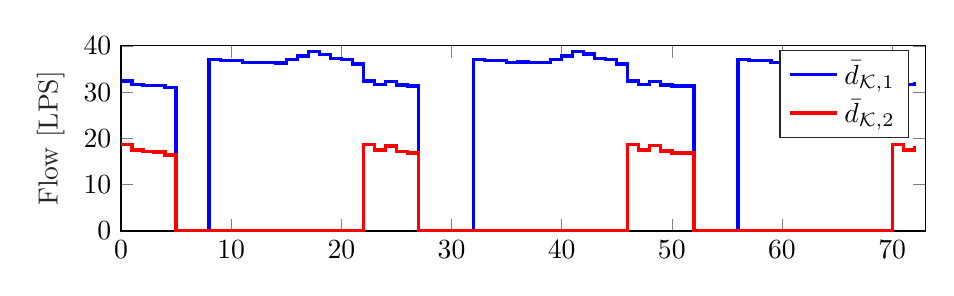
\begin{tikzpicture}

\begin{axis}[%
width=4.021in,
height=0.926in,
at={(0.75in,0.431in)},
scale only axis,
xmin=0,
xmax=73,
%xlabel style={font=\color{white!15!black}},
%xlabel={Time [h]},
ymin=0,
ymax=40,
ylabel style={font=\color{white!15!black}},
ylabel={Flow  [LPS]},
axis background/.style={fill=white},
legend style={legend cell align=left, align=left, draw=white!15!black}
]
\addplot[const plot, color=blue, line width=1.2pt] table[row sep=crcr] {%
0	32.41\\
1	31.67\\
2	31.44\\
3	31.42\\
4	31.03\\
5	0\\
6	0\\
7	0\\
8	37.09\\
9	36.88\\
10	36.76\\
11	36.37\\
12	36.46\\
13	36.4\\
14	36.31\\
15	37.04\\
16	37.78\\
17	38.7\\
18	38.19\\
19	37.19\\
20	37.02\\
21	36.06\\
22	32.4\\
23	31.67\\
24	32.26\\
25	31.53\\
26	31.3\\
27	0\\
28	0\\
29	0\\
30	0\\
31	0\\
32	37.11\\
33	36.9\\
34	36.78\\
35	36.38\\
36	36.48\\
37	36.42\\
38	36.33\\
39	37.05\\
40	37.8\\
41	38.71\\
42	38.21\\
43	37.21\\
44	37.04\\
45	36.07\\
46	32.42\\
47	31.68\\
48	32.27\\
49	31.54\\
50	31.31\\
51	31.29\\
52	0\\
53	0\\
54	0\\
55	0\\
56	37.1\\
57	36.9\\
58	36.77\\
59	36.38\\
60	36.48\\
61	36.41\\
62	36.32\\
63	37.05\\
64	37.8\\
65	38.71\\
66	38.21\\
67	37.2\\
68	37.04\\
69	36.07\\
70	32.42\\
71	31.68\\
72	32.27\\
};
\addlegendentry{$\bar{d}_{\mathcal{K},1}$}

\addplot[const plot, color=red, line width=1.2pt] table[row sep=crcr] {%
0	18.64\\
1	17.5\\
2	17.12\\
3	17.07\\
4	16.43\\
5	0\\
6	0\\
7	0\\
8	0\\
9	0\\
10	0\\
11	0\\
12	0\\
13	0\\
14	0\\
15	0\\
16	0\\
17	0\\
18	0\\
19	0\\
20	0\\
21	0\\
22	18.63\\
23	17.49\\
24	18.39\\
25	17.24\\
26	16.86\\
27	0\\
28	0\\
29	0\\
30	0\\
31	0\\
32	0\\
33	0\\
34	0\\
35	0\\
36	0\\
37	0\\
38	0\\
39	0\\
40	0\\
41	0\\
42	0\\
43	0\\
44	0\\
45	0\\
46	18.65\\
47	17.51\\
48	18.41\\
49	17.26\\
50	16.88\\
51	16.84\\
52	0\\
53	0\\
54	0\\
55	0\\
56	0\\
57	0\\
58	0\\
59	0\\
60	0\\
61	0\\
62	0\\
63	0\\
64	0\\
65	0\\
66	0\\
67	0\\
68	0\\
69	0\\
70	18.65\\
71	17.51\\
72	18.41\\
};
\addlegendentry{ $\bar{d}_{\mathcal{K},2}$}

\end{axis}
\end{tikzpicture}% 
 \vspace{-2.5mm}
 %\caption{Inlet flows of $PU_1$ and $PU_2$.}
 \label{fig:dk_sigma1}
 \end{figure}

 \vspace{-5mm}

   %WT - sigma1
 \begin{figure}[H]
 \centering
 \hspace{-4.5mm}
 %
\includegraphics[width=0.35\textwidth]{report/pictures/missingfigure}
 % This file was created by matlab2tikz.
%
%The latest updates can be retrieved from
%  http://www.mathworks.com/matlabcentral/fileexchange/22022-matlab2tikz-matlab2tikz
%where you can also make suggestions and rate matlab2tikz.
%
\definecolor{mycolor1}{rgb}{0.00000,0.44700,0.74100}%
%
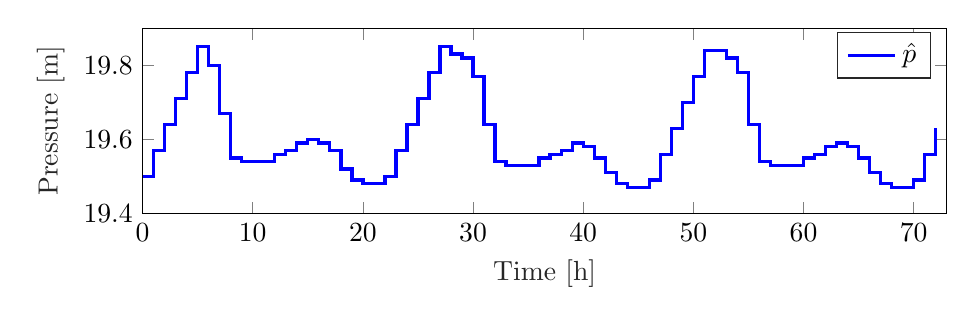
\begin{tikzpicture}

\begin{axis}[%
width=4.021in,
height=0.926in,
at={(0.792in,0.434in)},
scale only axis,
xmin=0,
xmax=73,
xlabel style={font=\color{white!15!black}},
xlabel={Time [h]},
ymin=19.4,
ymax=19.9,
ylabel style={font=\color{white!15!black}},
ylabel={Pressure  [m]},
axis background/.style={fill=white},
legend style={legend cell align=left, align=left, draw=white!15!black}
]
\addplot[const plot, color=blue, line width=1.2pt] table[row sep=crcr] {%
0	19.5\\
1	19.57\\
2	19.64\\
3	19.71\\
4	19.78\\
5	19.85\\
6	19.8\\
7	19.67\\
8	19.55\\
9	19.54\\
10	19.54\\
11	19.54\\
12	19.56\\
13	19.57\\
14	19.59\\
15	19.6\\
16	19.59\\
17	19.57\\
18	19.52\\
19	19.49\\
20	19.48\\
21	19.48\\
22	19.5\\
23	19.57\\
24	19.64\\
25	19.71\\
26	19.78\\
27	19.85\\
28	19.83\\
29	19.82\\
30	19.77\\
31	19.64\\
32	19.54\\
33	19.53\\
34	19.53\\
35	19.53\\
36	19.55\\
37	19.56\\
38	19.57\\
39	19.59\\
40	19.58\\
41	19.55\\
42	19.51\\
43	19.48\\
44	19.47\\
45	19.47\\
46	19.49\\
47	19.56\\
48	19.63\\
49	19.7\\
50	19.77\\
51	19.84\\
52	19.84\\
53	19.82\\
54	19.78\\
55	19.64\\
56	19.54\\
57	19.53\\
58	19.53\\
59	19.53\\
60	19.55\\
61	19.56\\
62	19.58\\
63	19.59\\
64	19.58\\
65	19.55\\
66	19.51\\
67	19.48\\
68	19.47\\
69	19.47\\
70	19.49\\
71	19.56\\
72	19.63\\
};
\addlegendentry{$\hat{p}$}

\end{axis}
\end{tikzpicture}% 
 \vspace{-2.5mm}
 \caption{Inlet flows of $PU_1$ and $PU_2$(above) and the pressure in the WT(below).}
 \label{fig:WT_sigma1}
 \end{figure}

 \vspace{-3mm}

For the two inlet pressures $\bar{p}_{\mathcal{K}1}$ and $\bar{p}_{\mathcal{K}2}$, the identification has been carried out with 12 RBF neurons. The performance goal has been chosen to the order of $10^{-4}$. \figref{fig:MSE_output} shows the mean of squared errors in terms of RBF neurons. 

   %MSE output
 \begin{figure}[H]
 \centering
 %\hspace{0mm}
 %
\includegraphics[width=0.35\textwidth]{report/pictures/missingfigure}
 % This file was created by matlab2tikz.
%
%The latest updates can be retrieved from
%  http://www.mathworks.com/matlabcentral/fileexchange/22022-matlab2tikz-matlab2tikz
%where you can also make suggestions and rate matlab2tikz.
%
\definecolor{mycolor1}{rgb}{0.92900,0.69400,0.12500}%
\definecolor{mycolor2}{rgb}{0.49400,0.18400,0.55600}%
%
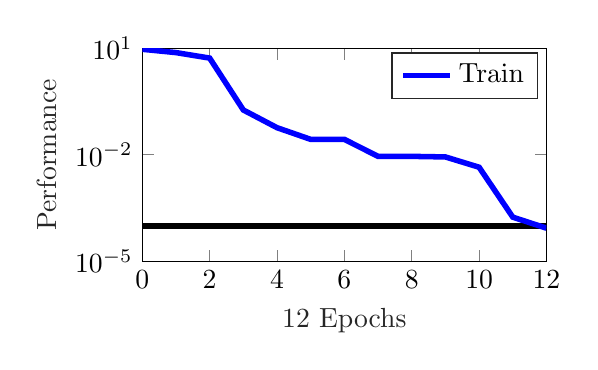
\begin{tikzpicture}

\begin{axis}[%
width=2.021in,
height=1.066in,
at={(0.758in,0.481in)},
scale only axis,
xmin=0,
xmax=12,
xlabel style={font=\color{white!15!black}},
xlabel={12 Epochs},
ymode=log,
ymin=1e-05,
ymax=10,
yminorticks=true,
ylabel style={font=\color{white!15!black}},
ylabel={Performance},
axis background/.style={fill=white},
%title style={font=\bfseries},
%title={Performance is 8.59528e-05, Goal is 0.0001},
legend style={legend cell align=left, align=left, draw=white!15!black}
]
\addplot [color=black, line width=2.0pt, forget plot]
  table[row sep=crcr]{%
0	0.0001\\
1	0.0001\\
2	0.0001\\
3	0.0001\\
4	0.0001\\
5	0.0001\\
6	0.0001\\
7	0.0001\\
8	0.0001\\
9	0.0001\\
10	0.0001\\
11	0.0001\\
12	0.0001\\
};
\addplot [color=blue, line width=2.0pt]
  table[row sep=crcr]{%
0	9.30084312163891\\
1	7.50455220664665\\
2	5.25664645000706\\
3	0.182039469478282\\
4	0.0578400961928023\\
5	0.0271025396912597\\
6	0.0271025396912595\\
7	0.00901207565548084\\
8	0.00901207565548112\\
9	0.00868579632596006\\
10	0.00445311736376068\\
11	0.000175417298503374\\
12	8.59528424540216e-05\\
};
\addlegendentry{Train}

\addplot [color=mycolor1, forget plot]
  table[row sep=crcr]{%
0	0\\
};
\addplot [color=mycolor2, forget plot]
  table[row sep=crcr]{%
0	0\\
};
\end{axis}
\end{tikzpicture}% 
 \vspace{-2.5mm}
 \caption{The network’s performance according to the mean of squared errors.}
 \label{fig:MSE_output}
 \end{figure}

 \vspace{-3mm}

As it is shown, a very good fit is achieved for a model which generalizes well the state equation. It is worth to mention that although more RBF neurons results in a more accurate fit, however it does not generalize so well the model as 12 RBF neurons do. In case of increasing the number of neurons, the identification resulted in overfit and the validation failed. The identification of $\bar{p}_{\mathcal{K}1}$ and $\bar{p}_{\mathcal{K}2}$ inlet pressures in case of $\sigma_1$ is shown in figref{}

\section{Identification and validation of the state equation}
\label{identification_and_validation_of_the_state_eq}  

abcd

\chapter{Example network description}
\label{physical_properties_example1}

\emph{In this part of the appendix, the corresponding physical parameters, control properties and consumption properties of the Multi-inlet, Single-WT example network are listed.}




